\documentclass[a4paper,12pt]{extarticle}
\usepackage[utf8x]{inputenc}
\usepackage[T1,T2A]{fontenc}
\usepackage[russian]{babel}
\usepackage{hyperref}
\usepackage{indentfirst}
\usepackage{listings}
\usepackage{color}
\usepackage{here}
\usepackage{array}
\usepackage{multirow}
\usepackage{graphicx}

\usepackage{caption}
\renewcommand{\lstlistingname}{Программа} % заголовок листингов кода

\bibliographystyle{ugost2008ls}

\usepackage{listings}
\lstset{ %
extendedchars=\true,
keepspaces=true,
language=C,						% choose the language of the code
basicstyle=\footnotesize,		% the size of the fonts that are used for the code
numbers=left,					% where to put the line-numbers
numberstyle=\footnotesize,		% the size of the fonts that are used for the line-numbers
stepnumber=1,					% the step between two line-numbers. If it is 1 each line will be numbered
numbersep=5pt,					% how far the line-numbers are from the code
backgroundcolor=\color{white},	% choose the background color. You must add \usepackage{color}
showspaces=false				% show spaces adding particular underscores
showstringspaces=false,			% underline spaces within strings
showtabs=false,					% show tabs within strings adding particular underscores
frame=single,           		% adds a frame around the code
tabsize=2,						% sets default tabsize to 2 spaces
captionpos=t,					% sets the caption-position to top
breaklines=true,				% sets automatic line breaking
breakatwhitespace=false,		% sets if automatic breaks should only happen at whitespace
escapeinside={\%*}{*)},			% if you want to add a comment within your code
postbreak=\raisebox{0ex}[0ex][0ex]{\ensuremath{\color{red}\hookrightarrow\space}},
texcl=true,
inputpath=listings,                     % директория с листингами
}

\usepackage[left=2cm,right=2cm,
top=2cm,bottom=2cm,bindingoffset=0cm]{geometry}

%% Нумерация картинок по секциям
\usepackage{chngcntr}
\counterwithin{figure}{section}
\counterwithin{table}{section}

%%Точки нумерации заголовков
\usepackage{titlesec}
\titlelabel{\thetitle.\quad}
\usepackage[dotinlabels]{titletoc}

%% Оформления подписи рисунка
\addto\captionsrussian{\renewcommand{\figurename}{Рисунок}}
\captionsetup[figure]{labelsep = period}

%% Подпись таблицы
\DeclareCaptionFormat{hfillstart}{\hfill#1#2#3\par}
\captionsetup[table]{format=hfillstart,labelsep=newline,justification=centering,skip=-10pt,textfont=bf}

%% Путь к каталогу с рисунками
\graphicspath{{fig/}}

%% Внесение titlepage в учёт счётчика страниц
\makeatletter
\renewenvironment{titlepage} {
 \thispagestyle{empty}
}
\makeatother


\begin{document}	% начало документа

% Титульная страница
\begin{titlepage}	% начало титульной страницы

	\begin{center}		% выравнивание по центру

		\large Санкт-Петербургский Политехнический Университет Петра Великого\\
		\large Институт компьютерных наук и технологий \\
		\large Кафедра компьютерных систем и программных технологий\\[6cm]
		% название института, затем отступ 6см
		
		\huge Базы данных\\[0.5cm] % название работы, затем отступ 0,5см
		\large Отчет по лабораторной работе №1\\[0.1cm]
		\large Разработка структуры БД\\[5cm]

	\end{center}


	\begin{flushright} % выравнивание по правому краю
		\begin{minipage}{0.25\textwidth} % врезка в половину ширины текста
			\begin{flushleft} % выровнять её содержимое по левому краю

				\large\textbf{Работу выполнил:}\\
				\large Графов Д.И.\\
				\large {Группа:} 33531/2\\
				
				\large \textbf{Преподаватель:}\\
				\large Мяснов А.В.

			\end{flushleft}
		\end{minipage}
	\end{flushright}
	
	\vfill % заполнить всё доступное ниже пространство

	\begin{center}
	\large Санкт-Петербург\\
	\large \the\year % вывести дату
	\end{center} % закончить выравнивание по центру

\thispagestyle{empty} % не нумеровать страницу
\end{titlepage} % конец титульной страницы

\vfill % заполнить всё доступное ниже пространство


% Содержание
% Содержание
\renewcommand\contentsname{\centerline{Содержание}}
\tableofcontents
\newpage




\section{Цель работы}
Познакомить студентов с возможностями реализации более сложной обработки данных на стороне сервера с помощью хранимых процедур.

\section{Программа работы}
\begin{itemize}
	\item Изучение возможностей языка PL/pgSQL.
	\item Создание двух хранимых процедур в соответствии с индивидуальным заданием, полученным у преподавателя.
	\item Выкладывание скрипта с созданными сущностями в репозиторий.
	\item Демонстрация результатов преподавателю.
\end{itemize}

\section{Теоретическая информация}
\subsection{PL/pgSQL}
PL/pgSQL (англ. Procedural Language/PostGres Structured Query Language) — процедурное расширение языка SQL, используемое в СУБД PostgreSQL. Этот язык предназначен для написания функций, триггеров и правил и обладает следующими особенностями:

\begin{itemize}
	\item добавляет управляющие конструкции к стандарту SQL;
	\item допускает сложные вычисления;
	\item может использовать все объекты БД, определенные пользователем;
	\item прост в использовании.
\end{itemize}

\subsection{Хранимая процедура}
Хранимая процедура — объект базы данных, представляющий собой набор SQL-инструкций, который компилируется один раз и хранится на сервере. Хранимые процедуры очень похожи на обыкновенные процедуры языков высокого уровня, у них могут быть входные и выходные параметры и локальные переменные, в них могут производиться числовые вычисления и операции над символьными данными, результаты которых могут присваиваться переменным и параметрам. В хранимых процедурах могут выполняться стандартные операции с базами данных (как DDL, так и DML). Кроме того, в хранимых процедурах возможны циклы и ветвления, то есть в них могут использоваться инструкции управления процессом исполнения.

\newpage
\section{Ход работы}
\subsection{Первое индивидуальное задание}
\textit{Для заданного бара и даты процедура выводит список доступных позиций на тот момент в баре. Считается, что товар, поставленный более, чем 2 недели назад, уже был распродан.}

Мной была написана функция get\_available(integer, timestamp), принимающая 2 параметра:
\begin{itemize}
	\item place\_id integer - для указания заведения (PK таблицы places);
	\item from\_date timestamp - для указания даты.
\end{itemize}

Функция возвращает таблицу, содержащую информацию о доступных позициях, а также даты поставки данных позиций.
Запрос, формирующий указанную таблицу, можно разделить на 2 части. Первая часть возвращает все поставки напитков из заданного заведения и за указанный промежуток времени. Вторая часть возвращает все поставки еды с теми же критериями.
Затем, с помощью оператора union, полученные подвыборки объединяются и возвращаются в качестве результата выполнения функции.

\lstinputlisting[
language=SQL,
caption={sp1.sql},
]{../../src/sp1.sql}

\begin{figure}[H]
	\begin{center}
		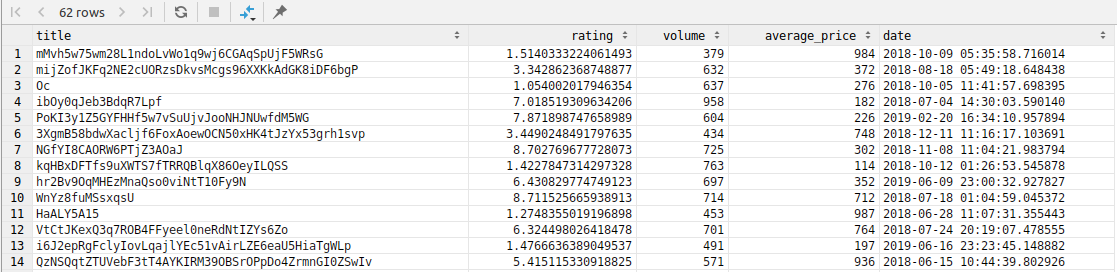
\includegraphics[scale=0.45]{sp1}
		\caption{Результат работы} 
		\label{pic:1} % название для ссылок внутри кода
	\end{center}
\end{figure}

\subsection{Второе индивидуальное задание}
\textit{Для заданного временного интервала процедура выводит перечень акций в каждом из баров в формате json:}
\begin{lstlisting}
{
	"bar title": [
		{
			"weekday": day,
			"discount": description of discount,
		},
		...
	],
	...
}
\end{lstlisting}

Пояснение: на данный момент структура БД не позволяет указать временной интервал проведения акции, поэтому данная функция не имеет параметров.

Написанная функция get\_discounts() создаёт таблицу disc, содержащую информащию о всех скидках во всех барах.
Затем, с помощью операторов json\_object\_agg и json\_build\_object, из данных таблицы disc формируется результат функции в формате json.

\lstinputlisting[
language=SQL,
caption={sp2.sql},
]{../../src/sp2.sql}

\begin{figure}[H]
	\begin{center}
		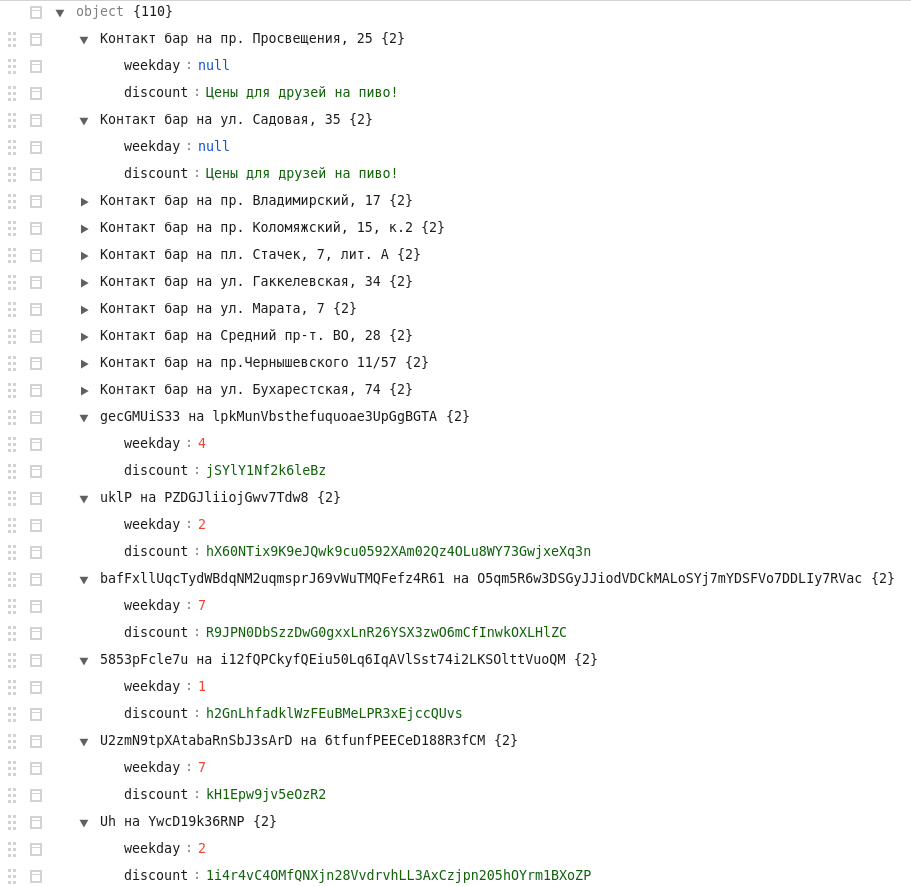
\includegraphics[scale=0.5]{sp2}
		\caption{Результат работы} 
		\label{pic:2} % название для ссылок внутри кода
	\end{center}
\end{figure}

\section{Выводы}
В ходе данной работы я ознакомился с процедурным языком PL/pgSQL, изучил его особенности и возможности, которые он предоставляет. Во время выполнения индивидуальных заданий я получил практические навыки по реализации обработки данных на стороне сервера с помощью хранимых процедур. Кроме того, я научился выводить результаты запросов в формате json.
\end{document}
